\documentclass[a4paper,twocolumn,9pt]{jsarticle} %% A4で9ptで二段組にします
\usepackage[dvipdfmx]{graphicx} %% 画像挿入のパッケージ

%% タイトル
\title{タイトル}

%% 著者名
\author{名前}

%% 日付
\date{日付} %% \todayで今日の日付に

%% 開始
\begin{document}

%% 表紙
\maketitle

%% 内容ごとにセクションを分ける
\section{はじめに}
研究背景とか

\section{次に}
どういう研究なのかとか

%% サブセクションでさらに分けれる
\subsection{その1}
1つ目

\subsection{その2}
2つ目

\section{さらにその次}
図\ref{fig1}のテスト
%% \ref{ラベル名}で図番号を参照できる

%% 図を入れる
\begin{figure}[htbp]
 \begin{center}
  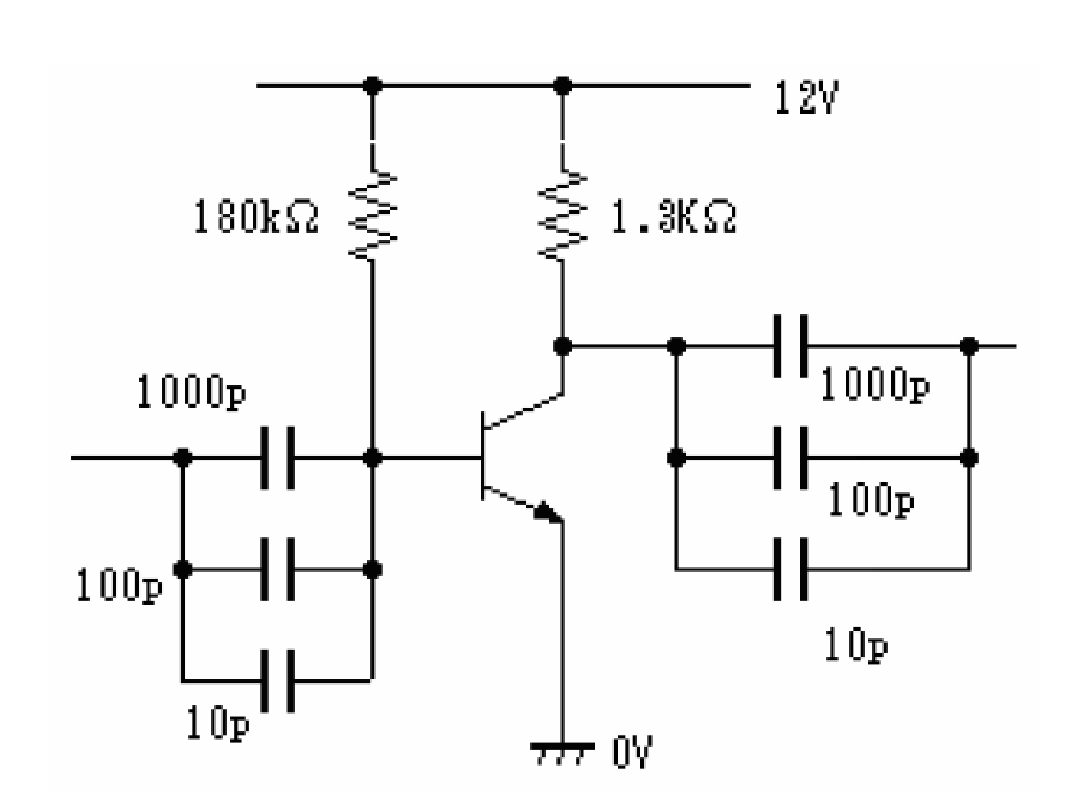
\includegraphics[clip,width=50mm]{fig.eps} %% includegraphics[scale=0.5]{~ で拡大縮小
   \caption{図題}
   \label{fig1}
 \end{center}
\end{figure}

\section{おわりに}
できたこととか今度について

参考文献\cite{bunken1}
%% \cite{名前}で文献を参照できる

%% 参考文献を載せる
\begin{thebibliography}{9}
 \bibitem{bunken1} 文献1
 \bibitem{bunken2} 文献2
 \bibitem{bunken3} 文献3
\end{thebibliography}

\end{document}
